\documentclass{article}
\pdfpagewidth=8.5in
\pdfpageheight=11in

\usepackage{../WMHreport}
% Use the postscript times font!
\usepackage{times}
\usepackage{soul}
\usepackage{url}
\usepackage{xcolor}
\usepackage{polski}
\usepackage[polish]{babel}
\usepackage[utf8]{inputenc}
\usepackage[T1]{fontenc}
\usepackage[utf8]{luainputenc}
\usepackage[hidelinks]{hyperref}
\usepackage[utf8]{inputenc}
\usepackage{caption}
\usepackage{indentfirst}
\usepackage{graphicx}
\usepackage{amsmath}
\usepackage{siunitx}
\usepackage{tabu}
\usepackage{booktabs}
\usepackage{float}
\usepackage{listings,newtxtt}
\lstset{basicstyle=\ttfamily, keywordstyle=\bfseries}
\usepackage{subfig}
\newcommand{\todo}[1]{\textcolor{red}{\textbf{TO DO:} #1}}
\newcommand{\solve}[1]{\textcolor{blue}{\textbf{SOLVE:} #1}}
\urlstyle{same}
	
\title{Współczesne metody heurysytczne\\ Sprawozdanie końcowe}

\author{
Julia Kłos, Jakub Sikora
\affiliations
numery albumów: 283607, 283418 \\
\emails
julia.klos.stud@pw.edu.pl, jakub.sikora2.stud@pw.edu.pl
}


\begin{document}
\maketitle

\section{Opis problemu}
\label{sec:problem}

Przedmiotem projektu jest znalezienie optymalnych parametrów maszyny wektorów nośnych (SVM-- \textit{Support Vector Machine}) w zagadnieniu aproksymacji. Aproksymowaną funkcją miała być dowolna ciągła funkcja dwuwymiarowa. W tym przypadku przyjęto funkcję określoną wzorem:

\begin{equation}
    \label{eqn:fun}
    f(x,y) = \log_{10}{|x|} \cos{y} + 0,55(x+y)
\end{equation}
\smallskip

\begin{figure}[h]
    \centering
    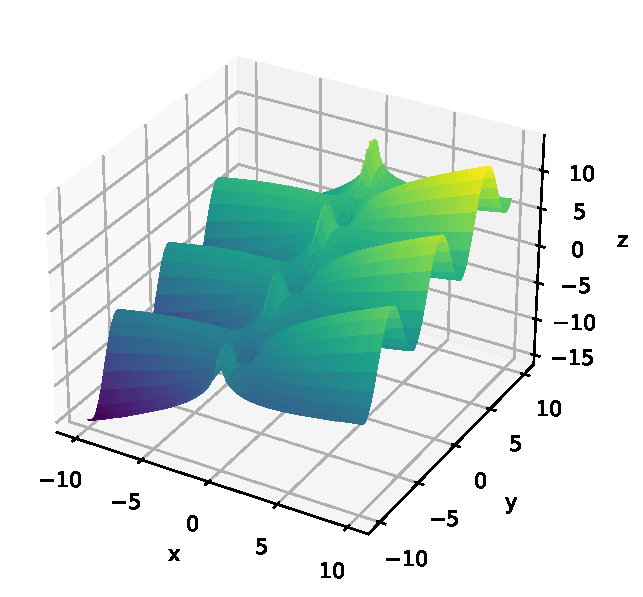
\includegraphics[width=0.5\textwidth]{assets/fun.pdf}
    \caption{Wykres aproksymowanej funkcji dwuwymiarowej}
    \label{fig:fun}
\end{figure}

W celu znalezienia optymalnych dla problemu parametrów zbadany zostanie wpływ poszczególnych parametrów algorytmu (funkcje jądrowe i ich atrybuty) na jakość regresji. Co więcej, aby sprawdzić, jak SVR (\textit{Support Vector Machine -- Regression}) poradziłby sobie dla rzeczywistych danych pomiarowych: zasymulowane zostaną one poprzez dodanie do aproksymowanej funkcji szumu. Zbadana zostanie jakość przybliżenia funkcji dla różnych poziomów szumu. Odporność przygotowanych modeli zostanie porównana z~innymi modelami regresji.

Jako miary oceny działania algorytmu wybrano:
\begin{itemize}
    \item błąd średniokwadratowy ($MSE$)
    \item średni błąd względny ($MAE$),
    \item współczynnik determinacji ($R^2$).
\end{itemize}

\begin{equation}
    \label{eqn:mse}
    MSE =\frac{1}{n} \sum_{i=1}^n (x_{i}-\hat{x}_{i})^2 \\[2ex]
\end{equation}
        
\begin{equation}
    \label{eqn:mae}
    MAE =\frac{1}{n} \sum_{i=1}^n \lvert x_{i}-\hat{x}_{i} \rvert \\[2ex]
\end{equation}
        
\begin{equation}
    \label{eqn:r2}
    R^{2} =1 - \frac{\sum_{i=1}^n (x_{i}-\hat{x}_{i})^2}{\sum_{i=1}^n (x_{i}-\bar{x}_{i})^2}   \\[2ex]
\end{equation}
        
\noindent
$\displaystyle
\begin{array}{ll}
              n      & \text{liczba pomiarów}\\
            x_{i} & \text{wartość rzeczywista}\\
            \hat{x}_{i} & \text{wartość przewidziana} \\
            \bar{x}_{i} & \text{wartość średnia} x
\end{array}
$ % opis problemu i aproksymowanej funkcji
\section{Opis algorytmów}
\label{sec:algorytm}

\subsection{SVM}
\label{subsec:svm}

\textit{Support Vector Machine}, czyli maszyna wektorów nośnych/podpierających, w podstawowej wersji stosowana jest do klasyfikacji poprzez znalezienie hiperprzestrzeni separującej z maksymalnym marginesem przykłady należące do różnych klas.

\begin{equation}
    y(x)= w^{T}x-b = 0
\end{equation}

Można zdefiniować równania decyzyjne:
\begin{equation}
    \begin{split}
    \label{eqn:decision}
     w^{T}x-b \geq 0,  d_{i}= +1\\
      w^{T}x-b < 0,  d_{i}= -1
     \end{split}
\end{equation}


\noindent
$\displaystyle
\begin{array}{ll}
    w      & \text{wektor wag}\\
    x & \text{wektor danych wejściowych} \\
    b & \text{polaryzacja} \\
    d \in \{+1,-1\} & \text{zdefiniowane klasy}
 \end{array}
$
 
Ostatecznie, całość może zostać zapisana w postaci nierówności:
 \begin{equation}
   d_{i}(w^{T}x-b) >=1
 \end{equation}
 
Spełniające je pary punktów $(x_{i}, d_{i})$ definiują wektory nośne (\textit{support vectors}), decydujące o położeniu hiperpłaszczyzny i szerokości marginesu separacji. Określenie decyzji wymaga wyznaczenia wektora wag oraz polaryzacji~\cite{zum}.
 
Można wykazać, że  maksymalna odległość pomiędzy marginesami (\ref{eqn:decision}) wynosi $M= \frac{2}{\| w \|}$.Rozwiązanie dąży do maksymalizacji marginesu M, co oznacza minimalizowanie wektora $w$. Zagadnienie optymalizacji sprowadza się do minimalizowania po $w$ wyrażenia 
\begin{equation}
\label{eqn:minimum2}
    \frac{1}{2}\| w \|^2.
\end{equation}

 
Dla problemów nieseparowalnych liniowo występuje konieczność zmniejszenia marginesu separacji, co można zapisać przy użyciu nierówności:

\begin{equation}
     d_{i}(w^{T}x-b)\geq 1 - \epsilon_{i} \
\end{equation}

W tym przypadku określa się granicę decyzyjną dodatkowo poprzez minimalizowanie wartości $\epsilon_{i}$. Dla parametru  generalizującego $C$, deklarowanego przez użytkownika, dąży się do minimalizacji wyrażenia:

\begin{equation}
    \frac{1}{2}\| w \|^2 + C\sum_{i=1}^n\epsilon_{i}
\end{equation}

\subsection{Funkcje jądrowe}
\label{subsec:kernel}

Większość spotykanych problemów nie jest jednak liniowo separowalna. Aby móc skorzystać, pomimo tego, z algorytmu SVM, należy skorzystać z możliwości przetransformowania danych do przestrzeni o innym wymiarze, w której dane z dużym prawdopodobieństwem będą separowane liniowo. Dla przypadku nieliniowego funkcja decyzyjna opisana może zostać równaniem:

\begin{equation}
 g(x) = w^{T}\phi(x)+b
 \end{equation}

Najczęściej wykorzystywane funkcje jądrowe to:
\begin{itemize}
    \item liniowa,
    \item wielomianowa,
    \item radialna (\textit{rbf}),
    \item sigmoidalna.
\end{itemize}
W tym zagadnieniu zazwyczaj wykorzystywana jest sztuczka jądrowa, która nie wymaga bezpośredniego transformowania atrybutów, a jedynie wyznaczania wartości funkcji jądrowej, bez definiowania nowych atrybutów.

\subsection{SVR}
\label{subsec:svr}

\textit{Support Vector Regression} (SVR) wykorzystuje te same reguły co SVM, jednak do rozwiązywania problemów związanych z aproksymacją funkcji. W regresji dąży się do minimalizowania błędu. Wykorzystując maszynę wektorów nośnych do tego zagadnienia, staramy się dopasować błąd do pewnego progu. Błąd jest minimalizowany (chociaż częściowo jest tolerowany), poprzez dopasowywanie hiperpłaszczyzny, maksymalizując margines.
 
W ramach projektu zbadany zostanie wpływ na wyniki regresji następujących parametrów:
\begin{itemize}
    \item wybranej funkcji jądrowej (liniowej, wielomianowej, radialnej i sigmoidalnej),
    \item parametr regularyzacji $C$,
    \item parametr marginesu błędu $\varepsilon$,
    \item parametr $\gamma$ (dla funkcji jądrowej: wielomianowej, radialnej i sigmoidalnej),
    \item stopień wielomianu $d$ (tylko wielomianowa),
    \item wyraz wolny $c_{0}$ (wielomianowa i~sigmoidalna).
\end{itemize}

\subsection{Algorytm ewolucyjny}
\label{subsec:evolution}
Algorytm ewolucyjny to metoda optymalizacyjna przeszukująca przestrzeń rozwiązań, którego idea została zaczerpnięta z ewolucji. Niezależnie od rozwiązywanego problemu, pojęcia związane z tą metodą zostały użyczone bezpośrednio z biologii. Kolejne generacje gatunku mają być jak najlepiej przystosowane do otaczającego środowiska, eliminując zaadaptowane osobniki. 

\textit{Osobniki}, czyli podstawowe jednostki (przykładowe rozwiązania) podlegające ewolucji, której celem jest stworzenie reprezentanta (znalezienie rozwiązania) możliwie najlepszego. \textit{Fenotypem} nazywamy wygląd zewnętrzy osobnika (czyli funkcja końcowa), a \textit{genotypem} zbiór informacji, stanowiący jego pełen opis. \textit{Populacja} to z kolei zespół osobników przebywających we wspólnym
środowisku. Genotyp jest stały w trakcie życia osobnika, a modyfikacje następują w wyniku rozmnażania. Fenotyp odzwierciedla dopasowanie osobnika do środowiska i to na jego podstawie dokonywana jest selekcja. Na zmiany w fenotypie wpływają zmiany w genotypie, które są głównie efektem krzyżowania osobników, chociaż mogą też wynikać z mutacji-- losowych, niewielkich zmian genotypu.

Algorytm rozpoczyna wybranie losowo pewnej populacji. Na podstawie ich dopasowania do środowiska, dokonywana jest selekcja-- najlepszym osobnikom umożliwia się reprodukcję. Genotypy wybranych osobników poddawane są krzyżowaniu, a dodatkowo losowo wprowadzane są mutacje. W ten sposób powstaje kolejne pokolenie, potencjalnie doskonalsze. Utrzymanie stałej liczby osobników w populacji umożliwia usuwanie najsłabszych osobników, ocenianych na podstawie fenotypu (funkcji go oceniającej). Jeśli nie zostanie spełnione kryterium stopu, powraca się do procesu reprodukcji.

Modyfikacje algorytmu ewolucyjnego uwzględniają różne definicje operacji krzyżowania, mutacji oraz selekcji. To co charakteryzuje tego typu algorytmy to szybkiego, równoległego przeszukiwania przestrzeni oraz uniknięcie pułapek minimum lokalnego.


\subsection{Reguły asocjacyjne}
\label{subsec:rules}
Do interpretacji uzyskanych wyników, wykorzystany zostanie algorytm \emph{apriori} do indukcji reguł asocjacyjnych~\cite{agrawal1996fast}. Reguły asocjacyjne opisują cechy zbioru danych powiązanych ze sobą w~pewien sposób. Każda reguła ma postać:

\begin{center}
    Jeżeli \emph{poprzednik}, to \emph{następnik} 
\end{center}

Z~każdą regułą można związać dwie miary: wsparcia oraz ufności. Miara wsparcia opisuje jak często w~danym zbiorze danych, w~jednej transakcji, występują zarówno poprzednik oraz następnik reguły. Ufność reguły opisuje prawdopodobieństwo warunkowe pojawienia się następnika reguły, pod warunkiem że wystąpił jej poprzednik.

Podstawowym algorytmem automatycznej indukcji reguł asocjacyjnych jest algorytm \emph{apriori}. Opiera się on na generacji częstych zbiorów, których wsparcie jest większe niż założony próg. Algorytm generuje drzewo zbiorów, odcinając co iterację wszystkie zbiory uznane za nieczęste. Dzięki przycinaniu, algorytm znacząco zmniejsza liczbę przejść przez cały zbiór danych w~celu policzenia wsparcia.

Aby wygenerować reguły asocjacyjne ze zbioru danych numerycznych, należy te dane zdyskretyzować oraz zamienić do formatu transakcyjnego. Zdecydowaliśmy się na wprowadzenie wprowadzenie sztucznego podziału wartości $$U = \{maly, sredni, duzy\},$$
dzięki czemu otrzymane reguły będą czytelne i~proste do interpretacji~\cite{agrawal1996fast}. % opis zastosowanych algorytmów
\section{Plan eksperymentów}
W~ramach projektu wykonane zostaną trzy eksperymenty:
\begin{itemize}
    \item badanie ogólnego zachowania wskaźników jakości w~zależności od parametrów funkcji jądrowych,
    \item optymalizacja parametrów funkcji jądrowej w~celu uzyskania jak najlepszego modelu,
    \item badanie wpływu szumu na jakość modelu.
\end{itemize}

W~celu zbadania ogólnego zachowania wskaźników jakości w~zależności od parametrów funkcji jądrowych, wykorzystany zostanie algorytm przeszukiwania zupełnego po przestrzeni dostępnych parametrów. Badana przestrzeń zostanie podzielona w~taki sposób aby rozważać tylko punkty o~różnych rzędach wielkości. Dla każdego zestawu parametrów zostanie przygotowany model SVR, którego wskaźniki jakości zostaną obliczone za pomocą pięciokrotnej walidacji krzyżowej.

Do interpretacji uzyskanych wyników, zostaną wykorzystane reguły asocjacyjne. Takie podejście pozwoli na automatyczne wyciągnięcie wniosków na temat pożądanych wartości poszczególnych parametrów, w~przypadku gdy nie będzie możliwym wykreślenie charakterystyki na wykresie.

W~drugim kroku, za pomocą algorytmu ewolucyjnego dokonamy optymalizacji parametrów ze względu na badane wskaźniki jakości. Korzystając z~wiedzy z~pierwszego eksperymentu, zawęzimy przedział poszukiwanych parametrów, tak aby ograniczyć ilość potrzebnych obliczeń do minimum. Dla każdej badanej funkcji jądrowej, proces optymalizacji zostanie przeprowadzony ze względu na jeden z~badanych wskaźników jakości: błąd średniokwadratowy, średni błąd względny oraz współczynnik determinancji.

Tematem ostatniego eksperymentu, będzie zbadanie działania zoptymalizowanych modeli w~obliczu zaszumionych danych. Na oryginalną funkcję~\ref{fig:fun} zostanie nałożony biały, addytywny, gaussowski szum o~różnych poziomach mocy. Dla każdego badanego poziomu, zostaną zbadane wskaźniki jakości zarówno na zbiorze trenującym jak i~zbiorze walidacyjnym. Celem tego eksperymentu będzie określenie dla jakiego poziomu szumu model zaczyna znacząco tracić na swojej jakości. % plan eksperymentów
\section{Badanie wpływu parametrów funkcji jądrowych na wskaźniki jakości modelu}
\label{sec:parametry}

Przeszukiwanie zupełne po przestrzeni parametrów, wraz z~5-krotną walidacją krzyżową zostało wykonane przy użyciu modułu \texttt{sklearn.model\_{}selection}, który udostępnia obiekt GridSearchCV. Na wejściu obiektu, podawany jest słownik z~parametrami, w~którym kluczem słownika jest nazwa parametru, natomiast wartością jest lista badanych parametrów. Podawane wartości różniły się między sobą o~rzędy wielkości, tak aby zbadać efektywnie jak największą przestrzeń.

\begin{lstlisting}[language=Python, captionpos=b, caption=Nagłówek klasy \texttt{GridSearchCV}]
class model_selection.GridSearchCV(
      estimator, param_grid, *, 
      scoring=None, n_jobs=None, 
      refit=True, cv=None, verbose=0, 
      pre_dispatch='2*n_jobs',
      error_score=nan, 
      return_train_score=False)
\end{lstlisting}

Generacja reguł asocjacyjnych zostanie wyjątkowo wykonana za pomocą języka R, wykorzystując do tego funkcję \textbf{apriori} z~pakietu~\textbf{arules}~\cite{arules}.

\begin{lstlisting}[language=R, captionpos=b, caption=Nagłówek funkcji \texttt{apriori}]
arules::apriori(data, 
                parameter = NULL, 
                appearance = NULL, 
                control = NULL)
\end{lstlisting}


Przeprowadziliśmy badania czterech funkcji jądrowych oraz wpływu ich parametrów na trzy różne wskaźniki jakości. W~tabeli~\ref{tab:modele} porównane zostały konkretne funkcje, badane parametry oraz liczbę policzonych modeli.

\begin{table}[htb]
    \centering
    \resizebox{\linewidth}{!}{%
    \begin{tabular}{||c c c||} 
        \hline
        funkcja jądrowa & parametry & liczba modeli \\ [0.5ex]
        \hline\hline
        liniowa & $C$, $\varepsilon$ & 125  \\ 
        \hline
        rbf & $C$, $\varepsilon$, $\gamma$ & 625 \\
        \hline
        wielomianowa & $C$, $\varepsilon$, $d$, $c_{0}$ & 3125 \\
        \hline
        sigmoidalna & $C$, $\varepsilon$, $\gamma$, $c_{0}$ & 3125 \\
        \hline 
    \end{tabular}}
    \caption{Porównanie parametrów badanych funkcji jądrowych oraz liczby wyuczonych modeli \label{tab:modele}}
\end{table}

Dla funkcji liniowej, która ma tylko dwa stopnie swobody, możliwym jest wykreślenie zależności danego wskaźnika jakości od parametrów $C$ oraz $\varepsilon$. Zależności te zostały wykreślone na rysunkach~\ref{fig:linear-mse} oraz~\ref{fig:linear-r2}.

\begin{figure}[htb]
    \centering
    \includegraphics[width=0.5\textwidth]{assets/linear-mse.pdf}
    \caption{Wartość wskaźnika MSE w~zależności od $C$ oraz~$\varepsilon$}
    \label{fig:linear-mse}
\end{figure}

\begin{figure}[htb]
    \centering
    \includegraphics[width=0.5\textwidth]{assets/linear-mae.pdf}
    \caption{Wartość wskaźnika MAE w~zależności od $C$ oraz~$\varepsilon$}
    \label{fig:linear-mae}
\end{figure}

\begin{figure}[htb]
    \centering
    \includegraphics[width=0.5\textwidth]{assets/linear-r2.pdf}
    \caption{Wartość wskaźnika $R^2$ w~zależności od $C$~oraz~$\varepsilon$}
    \label{fig:linear-r2}
\end{figure}

Dla wyników przeszukiwania odnoszących się do pozostałych funkcji jądrowych, z~racji zbyt dużej wymiarowości, wygenerowane zostały reguły asocjacyjne. Najciekawsze reguły zostały przedstawione w tabeli~\ref{tab:reguly}.

Kod realizujący przeszukiwanie zupełne po podanej przestrzeni parametrów został zamieszczony w~notatniku \texttt{Projekt-WMH.ipynb} natomiast analiza wyników została przeprowadzona w~notatniku \texttt{GridSearchResults.ipynb}. Indukcja reguł odbyła się przy użyciu języka~R, skrypt wykonujący to zadanie można znaleźć pod ścieżką \texttt{rules-induction/rules.R}.

\begin{table*}[t]
    \centering
    \resizebox{\linewidth}{!}{%
    \begin{tabular}{||c c c c||} 
        \hline
        poprzednik & następnik & wsparcie & ufność \\ [0.5ex]
        \hline\hline
        kernel=linear, C=small, epsilon=small & mean\_{}train\_{}mse=big & 0,133 & 0,666 \\ 
        \hline
        kernel=linear, C=small, epsilon=small & mean\_{}train\_{}mae=big & 0,133 & 0,666 \\ 
        \hline
        kernel=linear, C=small, epsilon=small & mean\_{}train\_{}r2=big & 0,133 & 0,666 \\ 
        \hline
        kernel=poly, C=big, coef0=small, degree=big, epsilon=small & mean\_{}test\_{}mae=small & 0,075 & 1,0 \\ 
        \hline
        kernel=poly, C=small, coef0=big, degree=small, epsilon=small & mean\_{}test\_{}mae=big & 0,05 & 1,0 \\ 
        \hline
        kernel=poly, C=big, coef0=big, degree=big, epsilon=small & mean\_{}fit\_{}time=big & 0,05 & 0,666 \\
        \hline
        kernel=rbf, C=big, epsilon=small, gamma=big & mean\_{}train\_{}mae=big & 0,144 & 1,0 \\
        \hline
        kernel=rbf, C=big, epsilon=small, gamma=big & mean\_{}test\_{}r2=big & 0,144 & 1,0 \\
        \hline
        kernel=rbf, C=big, epsilon=small, gamma=big & mean\_{}fit\_{}time=big & 0,144 & 1,0 \\
        \hline
        kernel=sigmoid, C=big, epsilon=small, coef0=small & mean\_{}train\_{}r2=big & 0,072 & 0,75 \\
        \hline
        kernel=sigmoid, C=small, epsilon=small, coef0=big & mean\_{}train\_{}mae=big & 0,064 & 0,666 \\
        \hline
        kernel=sigmoid, C=small, epsilon=small, gamma=small & mean\_{}fit\_{}time=big & 0,064 & 0,666 \\
        \hline
    \end{tabular}}
\caption{Najciekawsze odnalezione reguły asocjacyjne \label{tab:reguly}}
\end{table*}

Na podstawie tabeli~\ref{tab:reguly} można wyciągnąć wiele wniosków na temat wpływu parametrów modelu na jego jakość. Dla liniowej funkcji jądrowej, lepsze rezultaty uzyskamy przy mniejszych wartościach parametru $\varepsilon$, natomiast sama wartość parametru $C$, nie wpływa znacząco na wskaźniki jakości. 
Dla funkcji wielomianowej, wysoki zadany stopień wielomianu, znacznie utrudnia dopasowanie wektorów, co sprawia że średni czas uczenia jest bardzo duży.  % opis przeszukiwania przestrzeni parametrów
\section{Optymalizacja modeli algorytmem ewolucyjnym}
\label{sec:optymalizacja}

Na podstawie wyników z~poprzedniej sekcji, ustaliliśmy sensowne przedziały dla każdego badanego parametru i~następnie uruchomiliśmy proces optymalizacji algorytmem ewolucyjnym. W~tym celu wykorzystaliśmy gotową implementację algorytmu ewolucyjnego, zaimplementowanego w~bibliotece \textbf{scipy.optimize}~\cite{scipy}. Polecenie \textbf{differential\_{}evolution} pozwala na dokładne sterowanie procesem optymalizacji, ustawienie ograniczeń oraz podanie własnej funkcji celu, dzięki czemu możliwym jest badanie różnych, złożonych wskaźników jakości. 

\begin{lstlisting}[language=Python, captionpos=b, caption=Nagłówek funkcji \texttt{differential\_{}evolution}]
def optimize.differential_evolution(
    func, bounds, args=(), tol=0.01, 
    strategy='best1bin', maxiter=1000, 
    popsize=15, mutation=0.5, 
    seed=None, callback=None, 
    disp=False, polish=True, 
    recombination=0.7, atol=0)
\end{lstlisting}

Na podstawie reguł otrzymanych w~sekcji~\ref{sec:parametry}, przeprowadziliśmy eksperymenty dla wszystkich czterech funkcji jądrowych. W~tabelach~\ref{tab:optim-linear}, \ref{tab:optim-rbf}, \ref{tab:optim-poly} oraz~\ref{tab:optim-sigmoid} zamieszczone zostały wyniki procesu optymalizacji. Przedstawione wskaźniki jakości zostały obliczone na zbiorze testowym. Aby móc uzyskać wynik w~rozsądnym czasie, ustawiliśmy maksymalną liczbę iteracji, przez co nie wszędzie udało się osiągnąć minimum.

\begin{table}[htb]
    \centering
    \resizebox{\linewidth}{!}{%
    {\tabulinesep=1.2mm
   \begin{tabu} {|c|c|c|c|}
        \hline
        parametry & MAE & MSE & $R^2$ \\ [0.5ex]
        \hline\hline
        \parbox{2.5cm}{$C=64,76$ \\ $\varepsilon=6,793 \cdot 10^{-3}$} & $0,413$ & $0,247$ & $0,732$ \\ 
        \hline
        \parbox{2.5cm}{$C=21,62$ \\ $\varepsilon=1,343 \cdot 10^{-3}$} & $0,413$ & $0,2475$ & $0,732$ \\ 
        \hline
        \parbox{2.5cm}{$C=6,092$ \\ $\varepsilon=2,85\cdot 10^{-3}$} & $0,413$ & $0,2475$ & $0,732$ \\ 
        \hline
    \end{tabu}}}
    \caption{Wyniki procesu optymalizacji wskaźników jakości za pomocą algorytmu ewolucyjnego dla liniowej funkcji jądrowej}
    \label{tab:optim-linear}
\end{table}

\begin{table}[htb]
    \centering
    \resizebox{\linewidth}{!}{%
    {\tabulinesep=1.2mm
    \begin{tabu} {|c|c|c|c|}
        \hline
        parametry & MAE & MSE & $R^2$ \\ [0.5ex]
        \hline\hline
        \parbox{2.5cm}{ $C=7,7144$ \\ $\varepsilon=1,036 \cdot 10^{-2}$ \\ $\gamma=24,5761$ } & $8,892 \cdot 10^{-3}$ & $8,605 \cdot 10^{-5}$ & $0,99$ \\ 
        \hline
        \parbox{2.5cm}{$C=7,8973$ \\ $\varepsilon=2,07 \cdot 10^{-2}$ \\ $\gamma=30,1051$} & $1,8 \cdot 10^{-2}$ & $3,5 \cdot 10^{-4}$ & $0,99$ \\ 
        \hline
        \parbox{2.5cm}{$C=62,901$ \\ $\varepsilon=1,902\cdot 10^{-3}$ \\ $\gamma=21,7312$} & $7,844 \cdot 10^{-8}$ & $2,234 \cdot 10^{-4}$ & $0,99$ \\ 
        \hline
    \end{tabu}}}
    \caption{Wyniki procesu optymalizacji wskaźników jakości za pomocą algorytmu ewolucyjnego dla radialnej funkcji jądrowej}
    \label{tab:optim-rbf}
\end{table}

\begin{table}[htb]
    \centering
    \resizebox{\linewidth}{!}{%
    {\tabulinesep=1.2mm
   \begin{tabu} {|c|c|c|c|}
        \hline
        parametry & MAE & MSE & $R^2$ \\ [0.5ex]
        \hline\hline
        \parbox{2.5cm}{$C=89,2653$ \\ $\varepsilon=5,399\cdot 10^{-2}$ \\ $c_{0}=7,5099$} & $0,6553$ & $0,7438$ & $0,1973$ \\ 
        \hline
        \parbox{2.5cm}{$C=70,9637$ \\ $\varepsilon=1,422$ \\ $c_{0}=7,5099$} & $0,43$ & $0,282$ & $0,695$ \\ 
        \hline
        \parbox{2.5cm}{$C=50,368$ \\ $\varepsilon=1,5026$ \\ $c_{0}=0,8776$} & $0,435$ & $0,2839$ & $0,693$ \\ 
        \hline
    \end{tabu}}}
    \caption{Wyniki procesu optymalizacji wskaźników jakości za pomocą algorytmu ewolucyjnego dla sigmoidalnej funkcji jądrowej}
    \label{tab:optim-sigmoid}
\end{table}




\begin{table}[htb]
    \centering
    \resizebox{\linewidth}{!}{%
    {\tabulinesep=1.2mm
   \begin{tabu} {|c|c|c|c|}
        \hline
        parametry & MAE & MSE & $R^2$ \\ [0.5ex]
        \hline\hline
        \parbox{2.5cm}{$d=7$ \\ $C=52,4748$ \\ $\varepsilon=2,8316\cdot 10^{-3}$ \\  $c_{0}=9,45789$} & $5,941 \cdot 10^{2}$ & $6,029 \cdot 10^{5}$ & $-6,5\cdot 10^{5}$ \\ 
        \hline
        \parbox{2.5cm}{$d=6$ \\ $C=98,0516$ \\ $\varepsilon=1,403\cdot 10^{-2}$ \\ $c_{0}=9,8968$} & $3,103 \cdot 10^{1}$ & $1,4\cdot 10^{4}$ & $-1,52\cdot 10^{3}$ \\ 
        \hline
        \parbox{2.5cm}{$d=4$ \\ $C=0,34617$ \\ $\varepsilon=0,4113$ \\ $c_{0}=2,253$} & $0,3699$ & $0,2049$ & $0,778$ \\ 
        \hline
    \end{tabu}}}
    \caption{Wyniki procesu optymalizacji wskaźników jakości za pomocą algorytmu ewolucyjnego dla wielomianowej funkcji jądrowej}
    \label{tab:optim-poly}
\end{table}


Dla wszystkich czterech badanych funkcji jądrowych udało odnaleźć się zadowalające modele, aproksymujące zadaną funkcję. Zgodnie z~naszymi oczekiwaniami, najlepsze rezultaty udało się uzyskać dla funkcji radialnej. Wskaźniki $MSE$ oraz $MAE$ osiągnęły wartości bliskie zeru, natomiast wskaźnik $R^2$ osiągnął wartość bliską maksymalnej, czyli jedynce. 

Zaskakująco dobry wynik został uzyskany przez maszynę z~liniową funkcją jądrową. Wyniki wskaźników jakości odbiegają od najlepszych, jednak z~racji na prostotę modelu, czas zarówno uczenia jak i~obliczenia wyniku są najkrótsze ze wszystkich, co jest jego niewątpliwą zaletą. W~niektórych zastosowaniach, przykładowo w~systemach czasu rzeczywistego, parametry szybkościowe mogą być istotniejsze niż rzeczywista jakość modelu.

Nie wszystkie próby optymalizacji zakończyły się pełnym sukcesem. Dla funkcji wielomianowej oraz sigmoidalnej, nie udało się znaleźć takich zestawów parametrów, które skutecznie minimalizowałyby funkcję celu. W~przypadkach gdy udało się już znaleźć pewne minimum, to rzeczywista jakość modelu nie odbiegała znacznie od tej uzyskanej dla liniowej funkcji jądrowej. Fakt, iż funkcje te implikują znacznie większą złożoność modelu sprawia, że zgodnie z~zasadą brzytwy Ockhama, modele tego typu klasyfikujemy na końcu stawki, za modelami z~radialną i~liniową funkcją jądrową. % opis optymalizacji parametrów
\section{Badanie wpływu szumu na proces uczenia}
\label{sec:szum}

Do tej pory, proces uczenia i~weryfikacji modeli przebiegał na niezaszumionych danych. W~przypadku danych rzeczywistych, przykładowo zebranych przez pewne urządzenie pomiarowe, rzadko kiedy mamy do czynienia z~taką sytuacją. W~ramach kolejnego eksperymentu, przetestowaliśmy jakość obliczonych w~sekcji~\ref{sec:optymalizacja} modeli. Na oryginalną funkcję nałożyliśmy biały, addytywny, gaussowski szum, zgodnie z~poniższym wzorem:

\begin{equation}
    f'(x,y) = f(x,y) + X \qquad X \sim \mathcal{N}(0, \sigma)\smallskip
\end{equation}

Wartości zmiennej losowej $X$ zostały obliczone przy użyciu funkcji \texttt{normal} z~modułu \texttt{numpy.random}.

W~ramach eksperymentu, sprawdzone zostało jak zmieniają się wskaźniki jakości przy rosnącej wartości parametru~$\sigma$. Dodatkowo, zależność jakości maszyny wektorów nośnych od poziomu szumu zostanie porównana z~jakością innego modelu. Celem tego porównania jest próba weryfikacji tezy, iż modele SVR są bardziej odporne na szum, w~porównaniu do innych modeli regresji. Do porównania został wykorzystany zwykły model regresji liniowej, który został zaimplementowany w~bibliotece \textbf{scikit-learn}~\cite{scikit-learn}.

\begin{lstlisting}[language=Python, captionpos=b, caption=Nagłówek klasy \texttt{LinearRegression}]
class linear_model.LinearRegression(*, 
    fit_intercept=True, 
    normalize=False, 
    copy_X=True, n_jobs=None, 
    positive=False)
\end{lstlisting}

\begin{figure}[h]
    \centering
    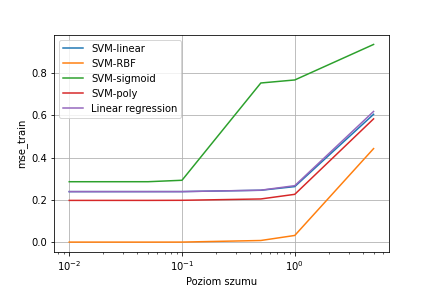
\includegraphics[width=1.1\columnwidth]{assets/mse_train.png}
    \caption{Wartość wskaźnika $MSE$ dla zbioru uczącego w~zależności od szumu}
    \label{fig:noise-mse-train}
\end{figure}

\begin{figure}[h]
    \centering
    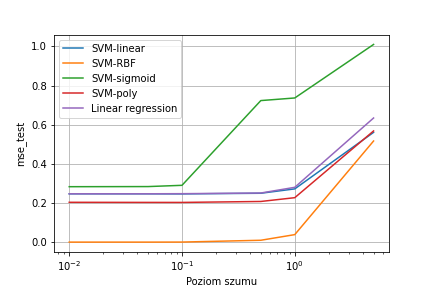
\includegraphics[width=1.1\columnwidth]{assets/mse_test.png}
    \caption{Wartość wskaźnika $MSE$ dla zbioru testowego w~zależności od szumu}
    \label{fig:noise-mse-test}
\end{figure}

%%%%%%%%%%%%%%%%%%%%%%%%%%%%%%%%%%%%%%%%%%%%%%%%%%%%%%%%%%%%%%%%%%%%%%%%%%%%%%%%

\begin{figure}[h]
    \centering
    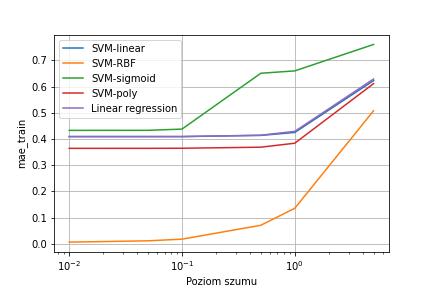
\includegraphics[width=1.1\columnwidth]{assets/mae_train.png}
    \caption{Wartość wskaźnika $MAE$ dla zbioru uczącego w~zależności od szumu}
    \label{fig:noise-mae-train}
\end{figure}

\begin{figure}[h]
    \centering
    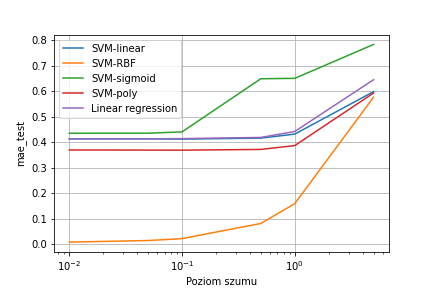
\includegraphics[width=1.1\columnwidth]{assets/mae_test.png}
    \caption{Wartość wskaźnika $MAE$ dla zbioru testowego w~zależności od szumu}
    \label{fig:noise-mae-test}
\end{figure}

%%%%%%%%%%%%%%%%%%%%%%%%%%%%%%%%%%%%%%%%%%%%%%%%%%%%%%%%%%%%%%%%%%%%%%%%%%%%%%%%

\begin{figure}[h]
    \centering
    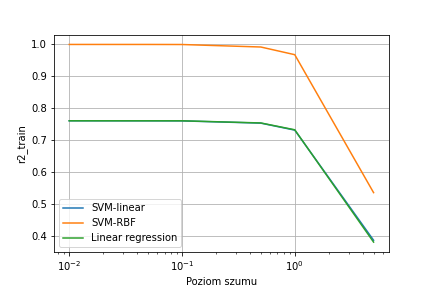
\includegraphics[width=1.1\columnwidth]{assets/r2_train.png}
    \caption{Wartość wskaźnika $R^2$ dla zbioru uczącego w~zależności od szumu}
    \label{fig:noise-r2-train}
\end{figure}

\begin{figure}[h]
    \centering
    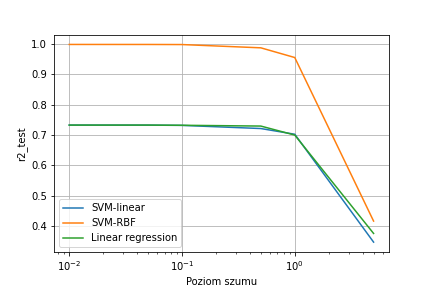
\includegraphics[width=1.1\columnwidth]{assets/r2_test.png}
    \caption{Wartość wskaźnika $R^2$ dla zbioru testowego w~zależności od szumu}
    \label{fig:noise-r2-test}
\end{figure}

Na rysunkach~\ref{fig:noise-mse-train}, \ref{fig:noise-mae-train} zostały przedstawione zależności trzech wskaźników jakości ($MSE$, $MAE$) od poziomu szumu $\sigma$ dla zbioru uczącego, a na rysunkach ~\ref{fig:noise-mse-test}, \ref{fig:noise-mae-test} odpowiednie zależności tych samych wskaźników dla zbioru testowego. Z problemem, niezależnie od poziomu szumu, zdecydowanie najgorzej poradził sobie SVM z sigmoidalną funkcją jądrową, co nie było zaskoczeniem ze względu na wyniki, które zostały zaprezentowane w \ref{sec:optymalizacja}. Dla tego typu modelu najszybciej wystąpiło znaczące pogorszenie wyników regresji. 

Zarówno dla $MSE$ jak i $MAE$ widać niezwykle podobieństwo osiąganych wyników pomiędzy maszyną wektorów nośnych o jądrze liniowym, a klasyczną regresją liniową. Różnica pomiędzy tymi modelami zaczyna być widoczna dla szumu rzędu jedności dla zbioru testowego z korzyścią dla SVR. Dla tych wskaźników niewiele gorzej wypadł SVM z wielomianową funkcją jądrową.

Zdecydowanie najlepiej z zadaniem uogólniania w zależności od szumu poradził sobie model maszyny wektorów nośnych z radialną funkcją jądrową. Warto tutaj jednak zauważyć, że dla szumu o $\sigma$ rzędu jedności to dla tego modelu występuje najbardziej gwałtowne pogorszenie wskaźników. 

Na rysunkach~\ref{fig:noise-r2-train}, oraz \ref{fig:noise-r2-test} zostały przedstawione zależności dla wskaźnika $R^2$ (determinacji) jedynie dla 3 modeli.  Dla SVM o funkcjach liniowych: sigmoidalnej i wielomianowej wyniki były na tyle złe ($R^2 < -2\times10^{5}$), że nie zostały tutaj zaprezentowane-- te modele nie radziły sobie z zaszumionymi danymi. Dla pozostałych modeli zależności pomiędzy jakością wyników regresji a szumem są podobne jak dla $MSE$ i $MAE$.
 % opis badań odporności na szum w danych
\section{Podsumowanie}
\label{sec:podsumowanie}

W~ramach projektu zbadano zagadnienie maszyny wektorów nośnych w~zagadnieniu regresji. Za pomocą przeszukiwania zupełnego, zbadano wpływ poszczególnych parametrów oraz zastosowanych funkcji jądrowych, na jakość modeli. Wiedza wyniesiona z~przeszukiwania, została zapisana w~postaci zbioru reguł asocjacyjnych. Na podstawie reguł, zawężono przedziały zainteresowań do optymalizacji parametrów, przeprowadzonej za pomocą algorytmu ewolucyjnego. Najlepsze modele zostały dodatkowo przetestowane na zaszumionych danych wejściowych, badając wpływ mocy szumu na jakość modelu. Wpływ mocy szumu na jakość modeli opartych o~SVM, został zestawiony z~wpływem szumu na inny, prosty model regresji. Ostatecznie, udało się uzyskać kilka modeli, które skutecznie mogłyby sobie poradzić z~zadaniem regresji, w~środowisku produkcyjnym.


\subsubsection{Wnioski}
\label{subsec:wnioski}
Maszyny wektorów nośnych są użytecznym narzędziem do tworzenia modeli, zarówno w~zadaniu klasyfikacji, jak i~regresji. Wyniki uzyskane w~sekcji~\ref{sec:szum}, potwierdzają postawioną tezę, iż modele te dobrze spisują się podczas pracy z~danymi obarczonymi szumem losowym. Potwierdziły się również nasze oczekiwania dotyczące radialnej funkcji jądrowej. Uzyskane wyniki, zarówno w~sekcji~\ref{sec:parametry}, jak i~w~sekcji~\ref{sec:optymalizacja}, jednoznacznie potwierdzają jej wyższość nad innymi funkcjami jądrowymi.

Bardzo pomocnym narzędziem w~uczeniu maszynowym okazują się mechanizmy optymalizacji. Dzięki przeszukiwaniu zupełnemu, udało nam się uzyskać bardzo dużą wiedzę (wyekstrahowaną automatycznie za pomocą reguł) na temat wpływu poszczególnych parametrów, na jakość modeli. Optymalizacja algorytmem ewolucyjnym, pozwoliła nam na dobór jak najlepszych wartości, tak aby móc uzyskać najlepsze możliwe wartości wskaźników jakości. 

Ważną kwestią w~optymalizacji jest niestety czas obliczeń. Dla bardziej złożonych funkcji jądrowych, uczenie modelu zajmuje bardzo dużo czasu, co skutecznie utrudnia przeprowadzanie procesu optymalizacji. Z~tego powodu, lepiej jest korzystać z~prostszych modeli, dla których możemy dobrać idealne parametry, niż z~bardziej złożonych, które potencjalnie mogą dać jeszcze lepsze wyniki, jednak znalezienie odpowiednich parametrów, które byłyby w~stanie zapewnić takie rezultaty, jest zadaniem zbyt czasochłonnym i~złożonym.
 % wnioski i podsumowanie projektu

\bibliographystyle{abbrv}
\bibliography{bibliography}
\end{document}